\chapter{Optimal Transport}%
\label{chapter:11}

\paragraph{Summary}
In this lecture we discuss optimal transport. After motivating the topic we
examine the discrete case where we show that discrete optimal transport can be
rewritten as a linear programming problem; more precisely, it can be rewritten
as a min-cost flow problem.

\section{Motivation}
Optimal transport is about finding the cost, and possibly the transport plan, to
transmogrify one distribution into another; one example is illustrated in the
Figure~\ref{fig:emd}.

\begin{wrapfigure}{r}{0.4\textwidth}
  \centering 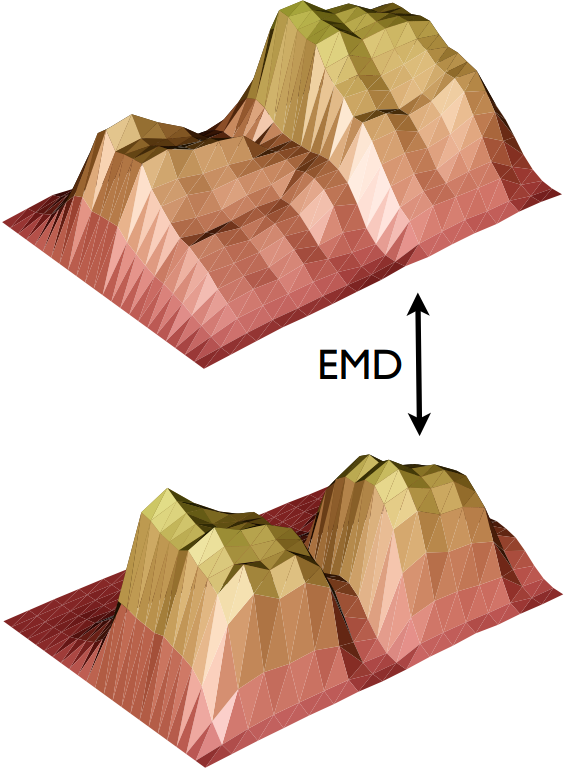
\includegraphics[width=0.38\textwidth]{Figures/emd}
  \caption{Transmogrifying one distribution into another. The transport cost is
    measured in terms of the earth mover's distance (EMD).}%
  \label{fig:emd}
\end{wrapfigure}

One important special case of this problem is when the bins have a spatial
layout, and the transport cost is a metric on that space. Another important
special case within this special case is when the cost is given by the Euclidean
distance in which case we call this cost the \emph{earth mover's distance}. In
this case the problem can be interpreted as to find the optimal strategy to move
one pile of dirt to somewhere else. Another example would be the optimal
transport plan of moving certain source items (\eg from a factory) to certain
target items (\eg to distribution centres). Of course, these examples can also
be generalised to continuous cases.

In the context of computer vision we can use optimal transport to measure the
discrepancy between different \emph{probability} distributions. This can be
used, for example, to decide for two pairs of distributions which of the pairs
are more similar to each other. A more concrete example is the automatic
generating of artificial images from given images, \eg generating images of bed
rooms or faces etc. The connection to optimal transport will be discussed later.
Optimal transport can also be used to interpolate between distribution. This
often yields better results than simple linear interpolation. This can be used
to interpolate between 3D shapes of objects (since they can be interpreted as
distributions) and to generate intermediate shapes that partly look like both of
the original shapes.

\section{Discrete Case}
As mentioned above, the goal is to transmogrify one distribution (the source)
into another distribution (the sink). If both the source and the sink are
discrete (\ie both are probability mass functions which are functions that give
the probability that a discrete random variable is exactly equal to some value),
then the problem can interpreted as a min-cost network flow problem which can be
efficiently solved using linear programming. If either of the distributions is
continuous (\ie it is a probability density function) the problem becomes harder
to solve. If both are continuous, the problem becomes yet harder although there
are certain special cases where it is easy to solve. We can visualise the task
as in Figure~\ref{fig:transport}.

\begin{figure}[htpb]
  \centering 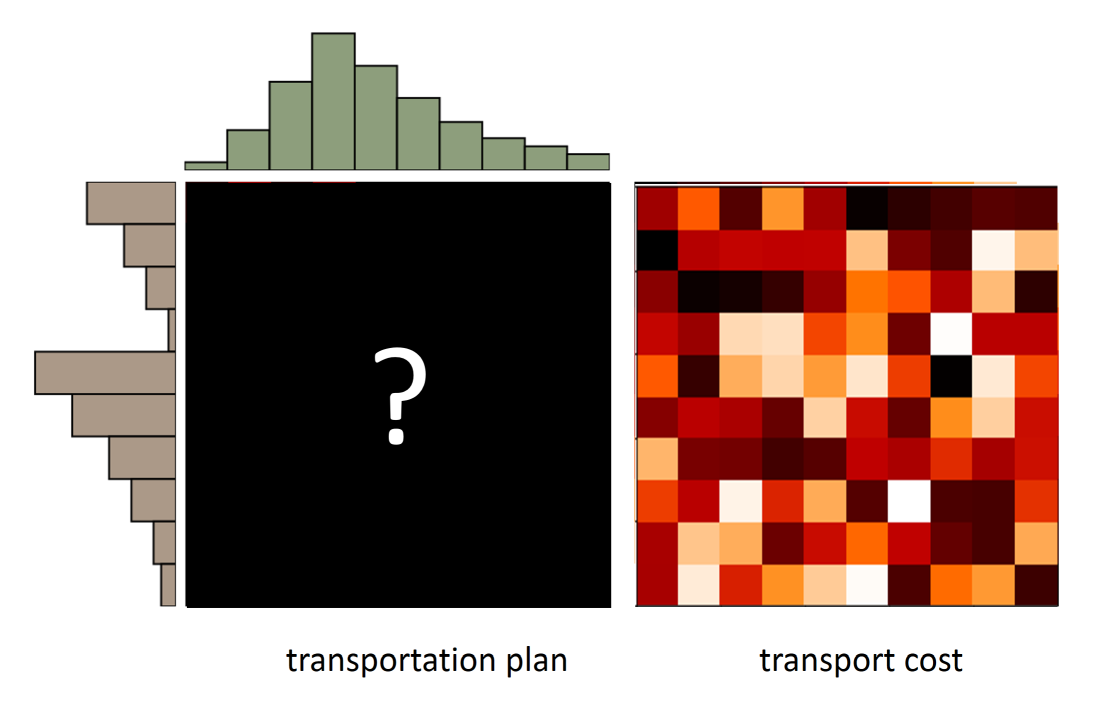
\includegraphics[width=0.7\textwidth]{Figures/transport}
  \caption{Examples for discrete distributions and transport cost matrix.}%
  \label{fig:transport}
\end{figure}

To derive the min-cost flow problem we assign vertices to each bin of the green
distribution and also to the bins of the red distribution (as was the case in
the previous chapter, we can duplicate these vertices to impose additional
constraints). The we connect the respective edges from one distribution to all
edges to the other distributions and set the cost of the new edges as given by
the cost matrix on the right. By now adding an additional source and one sink
node that connect to the first and the second distribution respectively, we have
converted our problem into a form that is similar to the one discussed in the
previous chapter which allows us to interpret it in terms of a linear program.

Alternatively we can the derive the linear programming formulation as follows.
Let $P \in \R^{n \times m}$ the flow matrix we want to find and let
$C \in \R^{n \times m}$ be the (given) cost matrix. The problem is now given by
\begin{align*}
  \text{Find }\ \min_P \ \sum_{i=1}^n \sum_{j=1}^m P_{ij} &C_{ij} \\
  \text{s.t. }\ \sum_{j=1}^m P_{ij} &= a_i \quad \forall i \\
  \sum_{i=1}^n P_{ij} &= b_j \quad \forall j \\
  \P_{ij} &\ge 0 \quad \forall i,j\,,
\end{align*}
where $a_i$ and $b_j$ are the values of the respective bins of the first and
second distribution, respectively. In other words, this is the amount that has
to be transported and so the first to constraints make sure that everything that
needs to be transported from the source does really get transported and that the
target receives everything it needs to receive. To make it clearer that this is
a linear program we first rewrite it as
\begin{align*}
  \text{Find }\ \min_{P \in \R^{n \times m}_{+}} \langle P,C \rangle \\
  \text{s.t. }\ P \mathbb{1}_m = a \quad \text{and} \quad P^\tp \mathbb{1}_n = b\,,
\end{align*}
where $\mathbb{1}_k$ is a $k$-dimensional vector containing only ones. By
identifying the matrices as vectors, we could also rewrite this again to obtain
the standard form of a linear program. This problem can now be solved using
standard linear programming solvers. Note, however, that it is usually more
efficient to directly use a solver that is specifically designed to solve
min-cost flow problems rather than a general LP solver. Alternatively, one can
use an algorithm that approximates the optimal transport solution which is
faster than the exact LP solver while yielding sufficiently accurate results.
One such algorithm is discussed in the next section.

\section{Wasserstein Generative Adversarial Networks (GANs)}
To conclude this Chapter, we briefly discuss a class of neural networks that can
be used to generate new images that are similar to training images that are
given to the network. To use the ideas from optimal transport discussed above we
first interpret the images as points in a high dimensional feature space that
are located on a manifold inside this space (for instance, the feature space
might be the space of images with $512 \times 512$ pixels and the manifold might
be the subset of images that show bed rooms). The basic idea of GANs is now as
follows. We want to use a neural network that tries to learn a probability
distribution on this manifold from which we can draw samples (\ie new artificial
examples of the given class of images). More precisely, the network only learns
a generator function that takes samples from a low-dimensional probability
distribution (\eg a 64-dimensional Gaussian) and maps them to the feature space.
To measure the discrepancy between our generated images and the training data we
cannot use the same ideas as we have used with CNNs since we have no ground
truth for the artificially generated images. Hence, we interpret the given
training data as a distribution in the feature space and do the same with a
number of images generated by our network and use the earth mover's distance as
a measure of discrepancy.

This, however, gives rise to a new problem: it is computationally costly to
compute the EMD in the high dimensional feature space. Luckily, this task can
also be well-approximated using another neural network. This is done by first
transforming the linear program discussed above into its associated dual
problem, which yields the same minimum as the original problem (we do not
discuss this duality in more detail here). This dual problem is then learned by
a neural network. That is, the loss function of the first network is (at least
partly) learned by a second network.

In summary, a Wasserstein GAN tries to find parameters of an decoder network
that maps samples from a primitive low-dimensional distribution to the space of
images such that the generated images have a small EMD to the real
images. However, the EMD itself is also learned by a second neural network and
this network and the decoder are trained simultaneously in an adversarial
manner.

%%% Local Variables:
%%% mode: latex
%%% TeX-master: "../main"
%%% End:
